\lecture{Data Analytics, Knime e Machine Learning}{20~-~01~-~2026}
%

%
\section{La nuova elettricità}
Così come l'elettricità trasformò ogni industria 100 anni fa, l'IA ha oggi il potenziale per trasformare ogni settore economico.
\begin{itemize}
    \item Intelligenza: La capacità mentale di apprendere dall'esperienza, adattarsi, gestire concetti astratti e manipolare l'ambiente;
    \item Intelligenza Artificiale (AI): La capacità di un computer digitale di svolgere compiti tipicamente associati agli esseri intelligenti (ragionamento, generalizzazione, apprendimento);
    \item Machine Learning (ML): Un sottoinsieme dell'IA. Invece di essere esplicitamente programmata per risolvere un problema, la macchina apprende dai dati per generare un modello. A riguardo rimando alla tabella \ref{tab:07-ml}.
\end{itemize}
%
\paragraph{Ma perché il Machine Learning è necessario?} È fondamentale quando l'esperienza umana non esiste, è inaffidabile, difficile da spiegare o quando la mole di dati è troppo elevata.

%
\section{Machine Learning}
Il ML è definito come la capacità di una macchina di apprendere dai dati senza essere esplicitamente programmata per un compito specifico. Vedi tabella \ref{tab:07-ml}.
\paragraph{Attenzione} Nelle slide è fornito un'esercitazione di laboratorio (poi da aggiungere nel project work) riguardo l'analisi di un braccio robotico con dei giunti: nelle prossime slide si farà riferimento a quest'ultimo. Vedere le slide del corso per informazioni, dati, file.

\begin{table}
    \centering
    \begin{tabular}{ll}%
        \toprule
        \textbf{Tradizionale}                           & \textbf{Machine Learning}                  \\
        \midrule
        $ \text{Dati} + \text{Code} \to \text{Output} $ & $ \text{Dati}+\text{Output}\to\text{Code}$ \\
        \bottomrule
    \end{tabular}
    \caption{}\label{tab:07-ml}
\end{table}

%
\subsection{Tipologie di Machine Learning}
Esistono due macro-categorie principali di apprendimento:
\begin{itemize}
    \item Supervised Learning;
    \item Unsupervised Learning.
\end{itemize}
%
\paragraph{Deep Learning} Utilizza reti neurali a più strati (hidden layers) per estrarre caratteristiche (features) sempre più astratte dai dati, imitando il cervello umano.

\subsubsection{Apprendimento supervisionato}
Utilizza dati ``etichettati'' (input + output corretto noto). Si divide in:
\begin{itemize}
    \item \emph{Regressione}: Predice un valore continuo (es. il prezzo di una casa basato sulla grandezza). L'obiettivo è trovare una funzione che approssimi la relazione tra variabili. Vedi figura \ref{fig:07-reg};
    \item \emph{Classificazione}: Assegna un'etichetta di classe discreta (es. ``gatto'' o ``cane'', ``guasto'' o ``funzionante'' \dots). Definisce un confine decisionale (\textbf{decision boundary}) tra i dati. Vedi figura \ref{fig:07-clas};
\end{itemize}
\begin{example}[Regressione]
    Regressione Lineare (retta), Polinomiale, Alberi di Regressione.
\end{example}
Vedi figura \ref{fig:07-appsup}.

\begin{figure}
    \centering
    \begin{subfigure}{0.45\linewidth}
        \centering
        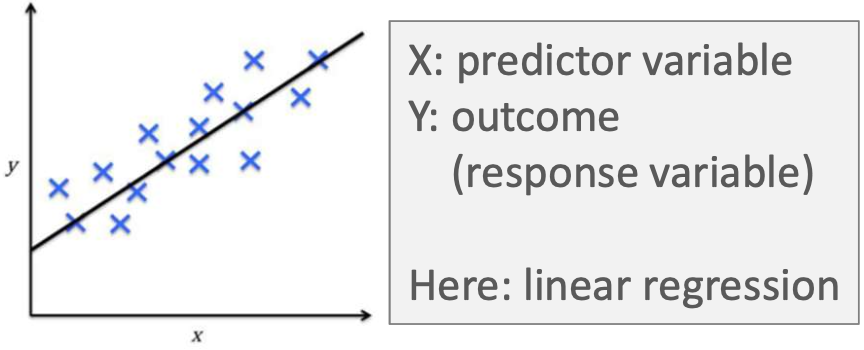
\includegraphics[width=\linewidth]{assets/Screenshot 2026-01-18 at 16.48.39.png}
        \caption{Regressione}\label{fig:07-reg}
    \end{subfigure}
    \begin{subfigure}{0.43\linewidth}
        \centering
        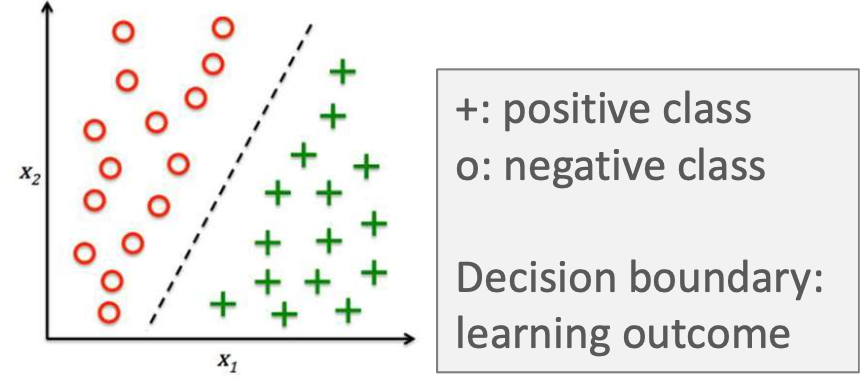
\includegraphics[width=\linewidth]{assets/Screenshot 2026-01-18 at 16.49.26.png}
        \caption{Classificazione}\label{fig:07-clas}
    \end{subfigure}
    \caption{Regressione e Classificazione nel Supervised Learning}\label{fig:}
\end{figure}
\begin{figure}
    \centering
    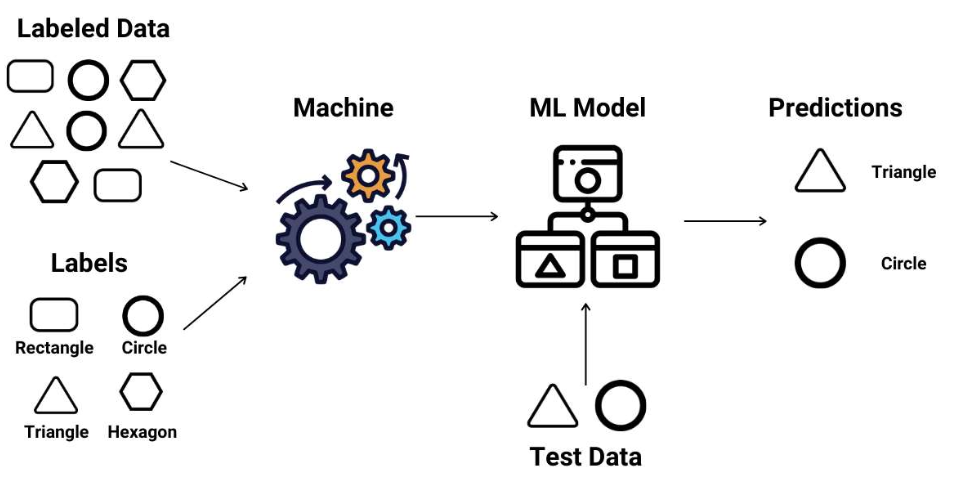
\includegraphics[width=0.6\linewidth]{assets/Screenshot 2026-01-18 at 16.46.27.png}
    \caption{Apprendimento supervisionato}\label{fig:07-appsup}
\end{figure}

\subsubsection{Apprendimento non supervisionato}
Utilizza dati non etichettati; l'algoritmo deve trovare strutture nascoste nei dati in modo autonomo.
\begin{itemize}
    \item \emph{Clustering}: Raggruppa istanze simili (es. segmentazione clienti). Massimizza la similarità intra-cluster e minimizza quella inter-cluster. Vedi grafico \ref{tikz:07-clustering};
    \item \emph{Anomaly Detection}: Identifica punti dati che non si conformano al comportamento standard (utile per guasti).
\end{itemize}
\begin{figure}[h]
    \centering
    % \resizebox{<larghezza>}{<altezza>}{<contenuto>}
    % Il '!' come altezza mantiene le proporzioni automaticamente
    \resizebox{0.6\linewidth}{!}{%
        \begin{tikzpicture}
            % --- Definizione Colori ---
            \definecolor{col1}{RGB}{231, 76, 60}
            \definecolor{col2}{RGB}{52, 152, 219}
            \definecolor{col3}{RGB}{46, 204, 113}
            \definecolor{colNoise}{RGB}{127, 140, 141}

            % --- Stili ---
            \tikzset{dataPoint/.style={circle, fill=#1, inner sep=0pt, minimum size=5pt}}
            \tikzset{clusterArea/.style={fill=#1, opacity=0.2, draw=#1, thick}}

            % --- Assi ---
            \draw[->, thick, gray!50] (-1,0) -- (7,0) node[right] {\small $x_1$};
            \draw[->, thick, gray!50] (0,-1) -- (0,6) node[above] {\small $x_2$};

            % --- Aree Cluster (Sfondo) ---
            \begin{scope}[on background layer]
                \draw[clusterArea=col1, rotate=20] (1.5, 1.5) ellipse (1.2 and 0.8);
                \draw[clusterArea=col2, rotate=-10] (5, 4.5) ellipse (1.1 and 0.9);
                \draw[clusterArea=col3] (5.5, 1) ellipse (1 and 0.7);
            \end{scope}

            % --- Punti Dati ---
            % Cluster 1
            \foreach \x/\y in {0.8/1.2, 1.2/1.8, 1.5/1.1, 1.9/1.6, 2.1/0.9, 1.0/1.5, 1.6/2.0}
                { \node[dataPoint=col1] at (\x,\y) {}; }
            % Cluster 2
            \foreach \x/\y in {4.2/4.8, 4.8/5.2, 5.5/4.9, 5.1/4.1, 5.8/4.5, 4.5/4.2}
                { \node[dataPoint=col2] at (\x,\y) {}; }
            % Cluster 3
            \foreach \x/\y in {4.8/0.8, 5.2/1.3, 5.8/0.9, 6.2/1.5, 6.5/0.7, 5.1/0.6}
                { \node[dataPoint=col3] at (\x,\y) {}; }
            % Rumore
            \foreach \x/\y in {3.5/3.0, 0.5/5.0, 6.5/3.0, 2.5/0}
                { \node[dataPoint=colNoise, minimum size=4pt] at (\x,\y) {}; }

            % --- Etichette ---
            \node[col1!80!black, font=\bfseries] at (1.5, 2.8) {Cluster 1};
            \node[col2!80!black, font=\bfseries] at (5.0, 6.0) {Cluster 2};
            \node[col3!80!black, font=\bfseries] at (5.5, -0.3) {Cluster 3};

        \end{tikzpicture}%
    } % Fine resizebox
    \caption{Esempio di clustering basato sulla densità.}
    \label{tikz:07-clustering}
\end{figure}
\begin{figure}[hpb]
    \centering
    % Definiamo stili comuni per coerenza tra i tre grafici
    \tikzset{
        axis/.style={->, >=stealth, thin, gray!80},
        data/.style={circle, fill=blue!60, inner sep=0pt, minimum size=3pt},
        anomaly/.style={circle, fill=red, inner sep=0pt, minimum size=4pt},
        model/.style={thick, color=red!80}
    }

    % --- GRAFICO 1: LINEAR REGRESSION ---
    \begin{subfigure}[b]{0.32\linewidth}
        \centering
        \resizebox{\linewidth}{!}{%
            \begin{tikzpicture}
                \draw[axis] (0,0) -- (4.2,0) node[right, scale=0.7]{$x$};
                \draw[axis] (0,0) -- (0,4.2) node[above, scale=0.7]{$y$};

                % Dati che seguono una linea
                \foreach \x/\y in {0.5/0.8, 1/1.2, 1.3/1.6, 2/2.1, 2.5/2.4, 3/3.2, 3.5/3.4, 3.8/3.9}
                \node[data] at (\x,\y) {};

                % Linea di regressione
                \draw[model] (0,0.5) -- (4,4);
            \end{tikzpicture}}
        \caption{Linear Regression}
        \label{fig:lin_reg}
    \end{subfigure}
    \hfill % Spazio flessibile tra le figure
    % --- GRAFICO 2: REGRESSION TREE (Step Function) ---
    \begin{subfigure}[b]{0.32\linewidth}
        \centering
        \resizebox{\linewidth}{!}{%
            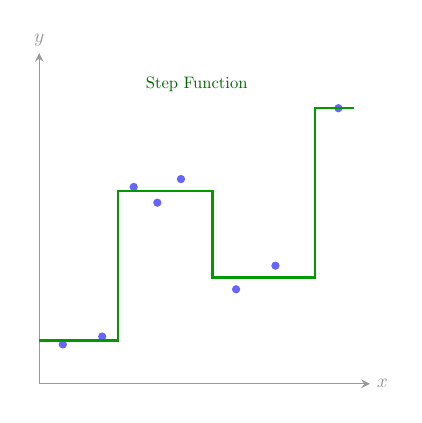
\begin{tikzpicture}
                \draw[axis] (0,0) -- (4.2,0) node[right, scale=0.7]{$x$};
                \draw[axis] (0,0) -- (0,4.2) node[above, scale=0.7]{$y$};

                % Dati sparsi (non lineari)
                \foreach \x/\y in {0.3/0.5, 0.8/0.6, 1.2/2.5, 1.5/2.3, 1.8/2.6, 2.5/1.2, 3.0/1.5, 3.8/3.5}
                \node[data] at (\x,\y) {};

                % Funzione a gradini (tipica degli alberi)
                \draw[model, color=green!60!black] (0,0.55) -- (1,0.55) -- (1,2.45) -- (2.2,2.45) -- (2.2,1.35) -- (3.5,1.35) -- (3.5,3.5) -- (4,3.5);
                \node[scale=0.6, green!40!black] at (2, 3.8) {Step Function};
            \end{tikzpicture}}
        \caption{Regression Tree}
        \label{fig:reg_tree}
    \end{subfigure}
    \hfill
    % --- GRAFICO 3: ANOMALY DETECTION ---
    \begin{subfigure}[b]{0.32\linewidth}
        \centering
        \resizebox{\linewidth}{!}{%
            \begin{tikzpicture}
                \draw[axis] (0,0) -- (4.2,0) node[right, scale=0.7]{$x_1$};
                \draw[axis] (0,0) -- (0,4.2) node[above, scale=0.7]{$x_2$};

                % Cluster Normale
                \draw[dashed, gray] (2,2) circle (1.2cm);
                \foreach \x/\y in {1.5/2, 2/2.2, 2.3/1.8, 1.8/2.5, 2.2/1.5, 1.6/1.6, 2.5/2.1, 1.9/1.9}
                \node[data] at (\x,\y) {};

                % Anomalie
                \node[anomaly] at (3.8, 3.8) {};
                \node[anomaly] at (0.5, 3.5) {};
                \node[anomaly] at (3.5, 0.8) {};

                \node[scale=0.6, red] at (3.8, 3.5) {Outlier};
            \end{tikzpicture}}
        \caption{Anomaly Detection}
        \label{fig:anomaly}
    \end{subfigure}

    \caption{Confronto visuale tra tre approcci di Machine Learning.}
    \label{fig:ml_comparison}
\end{figure}
%
\subsection{Workflow Machine Learning nel Digital Twin}
L'integrazione dell'AI nel Digital Twin segue un processo ciclico:
\begin{enumerate}
    \item Raccolta e pulizia dati: Creazione di un dataset affidabile (inclusi dati di guasto);
    \item Training: Addestramento del modello per minimizzare l'errore (es. usando reti neurali);
    \item Valutazione e Test: Verifica su dati non usati nel training (test set).
\end{enumerate}
%
\paragraph{Goodness of fit} Bisogna trovare il giusto passo per l'addestramento ed il testing dell'IA:
\begin{itemize}
    \item Underfitting: Il modello è troppo semplice e non impara né dal training né dal test set;
    \item Overfitting: Il modello ``impara a memoria'' i dati di training ma fallisce sui nuovi dati (test set);
    \item Appropriate fit: Il modello perfoma in modo ottimale sia nel training set che nel test set.
\end{itemize}

%
\section{Piattaforma Knime}
KNIME è una piattaforma open-source per la Data Science basata su un paradigma di programmazione visiva.
%
\subsection{Workflow}
Knime è una pipeline di ``nodi'', i dati scorrono da sinistra a destra.
%
\paragraph{Nodi} Sono le unità di elaborazione. Ogni nodo ha un semaforo di stato:
\begin{itemize}
    \item \emph{Rosso}: Non configurato;
    \item \emph{Giallo}: Configurato;
    \item \emph{Verde}: Eseguito (dati pronti all'uscita).
\end{itemize}

%
\paragraph{Porte} I nodi si collegano solo se le porte sono dello stesso tipo (es. dati tabellari, modelli ML \dots).

%
\subsection{Data Preparation}
Come visto in precedenza, il processo di Machine Learning inizia sempre con la gestione dei dati. Nel caso studio proposto (vedi slide), vengono applicati i seguenti passaggi fondamentali:
\begin{enumerate}
    \item Importazione: Utilizzo del nodo CSV Reader per caricare i dati;
    \item Pulizia (Data Cleaning):
          \begin{itemize}
              \item \emph{Column Filter}: Selezione delle variabili di interesse (Speed, Current, Position Target);
              \item \emph{Row Filter}: Rimozione delle righe contenenti valori mancanti (missing values).
          \end{itemize}
    \item Analisi degli Outlier (Box Plot): Si utilizza il Box Plot per visualizzare la distribuzione (minimo, massimo, mediana, quartili) e individuare valori anomali;
    \item Normalizzazione: Fondamentale quando le variabili hanno scale numeriche diverse (es. intesità di corrente (\SI{}{\ampere}), potenziale elettrico (\SI{}{\volt}), velocità ( $\frac{m}{s} $) \dots). Si usa il nodo Normalizer. Vedi la sezione \ref{subsubsec:norm} per approfondimenti.
    \item Correlazione: Si usa la Linear Correlation per identificare variabili ridondanti o influenti. Valori vicini a $ +1 $ o $ -1 $ indicano forte correlazione, $ 0 $ indica nessuna correlazione.
\end{enumerate}

\subsubsection{Normalizzazione} \label{subsubsec:norm}
%
\paragraph{Min-Max} Scala i dati in un range [$ \min_{A} $, $ \max_{A} $]. Garantisce che tutte le feature abbiano la stessa scala ma non gestisce bene gli outlier.

Avendo un $ \min_{a} $ ed un $ \max_{a} $, siano definiti come $ \min_{A} $ e $ \max_{A} $ i nuovi valori di minimo e di massimo, scalando verso $ \min_{A} $, $ \max_{A} $ si ottiene:
\[
    v^{\prime}=\frac{v-min}{max_{a}-min_{a}}(max_{A}-min_{A})+min_{A}
\]
%
\paragraph{Z-Score} Gestisce meglio gli outlier usando media $\mu$ e deviazione standard $\sigma$:
\[
    v^{\prime}=\frac{v-\mu_{A}}{\sigma_{A}}
\]

%
\subsection{Unsupervised Clustering}
Ora confrontiamo due algoritmi per raggruppare i dati di corrente e velocità:
\begin{itemize}
    \item k-Means;
    \item DBSCAN (Density-Based Spatial Clustering of Applications with Noise).
\end{itemize}

\subsubsection{k-Means}
Richiede di specificare il numero di cluster $k$ a priori, funziona iterativamente ricalcolando i centroidi.
\\Nel Case Study troviamo come risultato: $R^2 \approx 0,773$: significa che tende a forzare cluster anche dove non esistono separazioni nette.
\subsubsection{DBSCAN}
È basato sulla densità, richiede due parametri: raggio $\epsilon$ e numero minimo di punti. Identifica Core Points e gestisce il rumore (outlier) e non richiede di definire il numero di cluster a priori.
\\Nel Case Study il risultato è simile al k-Means: $R^2 \approx 0,774$, ma con tempi di esecuzione più lunghi.

%
\subsection{Supervised Regression}
L'obiettivo è predire la Corrente (variabile dipendente $Y$) basandosi sulla Velocità (variabile indipendente $X$).
Un passaggio critico è il \emph{Partitioning}: i dati vengono divisi in 50\% per il training (costruzione modello) e 50\% per il testing (validazione). Vedi figura \ref{fig:10-reg}.
%
\paragraph{Linear Regression:} Cerca la migliore linea retta che minimizza l'errore quadratico ($Y = P_{0} + P_{1X} + \epsilon$).

Il modello ha come risultato $R^2=0,783 $: approssima il trend medio ma fallisce nel catturare le variazioni locali complesse, mostrando molti errori locali.

%
\paragraph{Regression Tree:} Partiziona i dati in sottoinsiemi omogenei attraverso una struttura ad albero (split iterativi basati su regole \verb|if-then|) ed è in grado di modellare funzioni non lineari (approssimazione a gradini).

Il risultato del modello è nettamente superiore, con $R^2=0,961$, un errore quadratico medio (MSE) molto più basso ($ 0,038 $ contro $ 0,213 $ della regressione lineare). Il grafico mostra che l'albero segue molto meglio la forma dei dati.

\begin{figure}
    \centering
    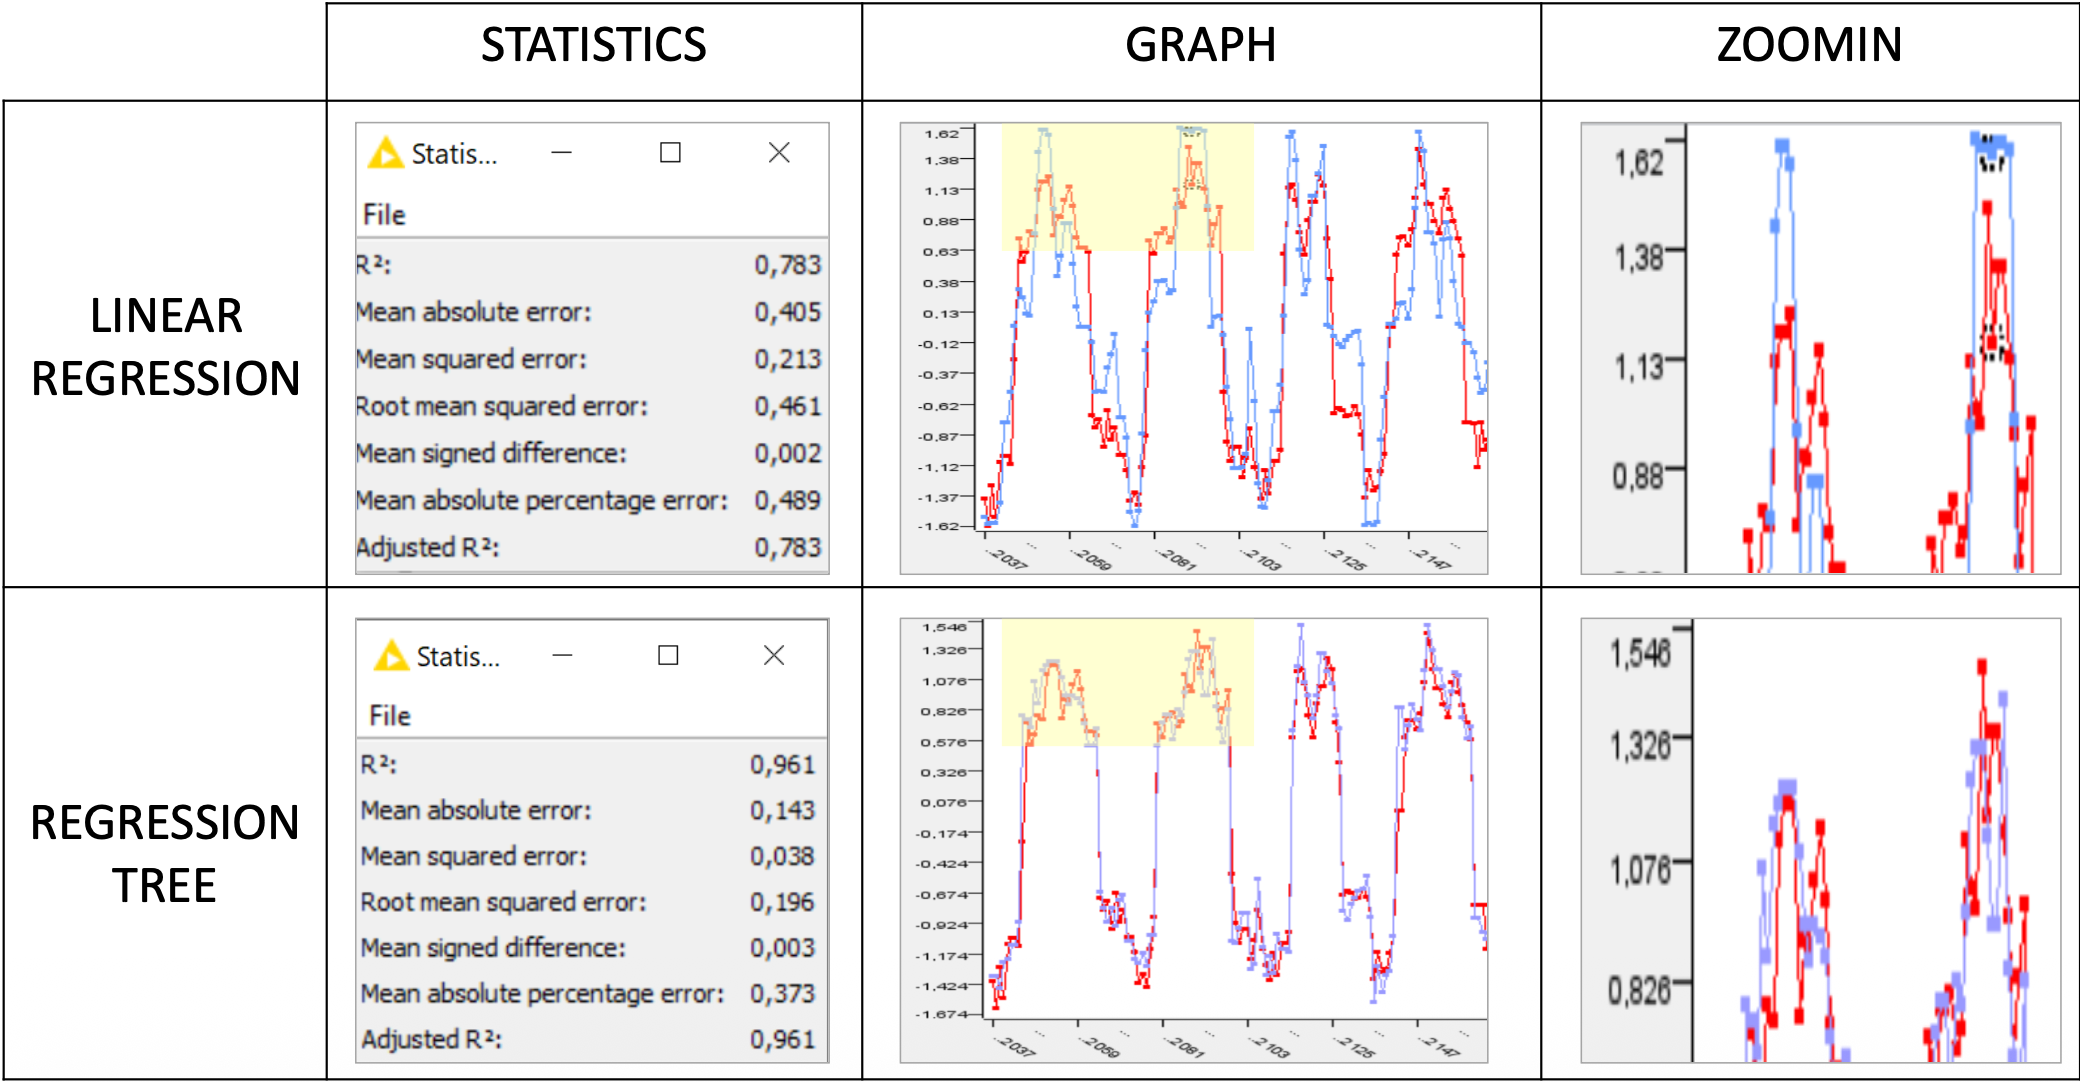
\includegraphics[width=0.9\linewidth]{assets/Screenshot 2026-01-20 at 17.44.01.png}
    \caption{Confronto tra i due tipi di regressione}\label{fig:10-reg}
\end{figure}